(2.25) \underline{例}。

设 $k$ 是代数闭域，$E_n$ 是 $k$ 上的仿射 $n$-维空间。设 $C$ 是 $E_n$ 中在原点处有奇点的约化曲线。赋予此奇点一个\underline{Enriques 图}（参见 [3]）：其顶点是 $C$ 上与原点无限邻近的点（2.4 和 2.15），将每个顶点与邻接于它的各顶点用线连接（2.5 和 2.15）。此图确定这些点在 $C$ 上的重数（2.11 和 2.18），并在 $n=2$ 时确定 $C$ 在原点处的奇点的不变量 $\delta$（2.10 和 2.11）。

对最简单的平面奇点，得到下表。顶点旁的数字表示其重数。

\begin{center}
\small
\setlength{\tabcolsep}{5pt}
\renewcommand{\arraystretch}{1.35}
\begin{tabular}{c c c c}
\textit{示意图} & \textit{方程} & $\delta$ & \textit{Enriques 图} \\

\begin{tikzpicture}[baseline=-.5ex,x=.55cm,y=.55cm]
  \draw[line width=.45pt] (-.8,0)--(.8,0);
\end{tikzpicture}
& $y=0$ & $0$ &
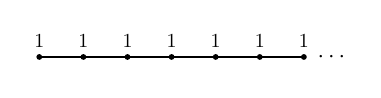
\begin{tikzpicture}[baseline=-.5ex,x=.56cm,y=.56cm]
  \foreach \x in {0,...,6}{
    \fill (\x,0) circle (1.05pt);
    \node[above=1pt,scale=.72] at (\x,0) {$1$};
  }
  \draw (0,0)--(6,0);
  \node[right=2pt,scale=.85] at (6,0) {$\cdots$};
\end{tikzpicture}
\\

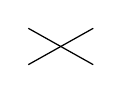
\begin{tikzpicture}[baseline=-.5ex,x=.55cm,y=.55cm]
  \draw[line width=.45pt] (-.75,-.42)--(.75,.42);
  \draw[line width=.45pt] (-.75,.42)--(.75,-.42);
\end{tikzpicture}
& $xy=0$ & $1$ &
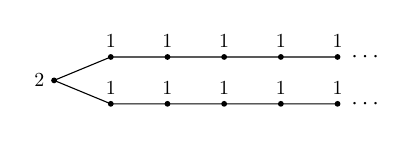
\begin{tikzpicture}[baseline=-.5ex,x=.72cm,y=.62cm]
  \fill (0,0) circle (1.05pt);
  \node[left=1pt,scale=.72] at (0,0) {$2$};
  \foreach \x in {1,...,5}{
    \fill (\x,.48) circle (1.05pt);
    \fill (\x,-.48) circle (1.05pt);
    \node[above=1pt,scale=.72] at (\x,.48) {$1$};
    \node[above=1pt,scale=.72] at (\x,-.48) {$1$};
  }
  \draw (0,0)--(1,.48)--(5,.48);
  \draw (0,0)--(1,-.48)--(5,-.48);
  \node[right=2pt,scale=.85] at (5,.48) {$\cdots$};
  \node[right=2pt,scale=.85] at (5,-.48) {$\cdots$};
\end{tikzpicture}
\\

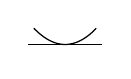
\begin{tikzpicture}[baseline=-.5ex,x=.55cm,y=.55cm]
  \draw[line width=.45pt] (-.85,0)--(.85,0);
  \draw[line width=.45pt,domain=-.72:.72,samples=40]
    plot (\x,{.72*\x*\x});
\end{tikzpicture}
& $y(y-x^2)=0$ & $2$ &
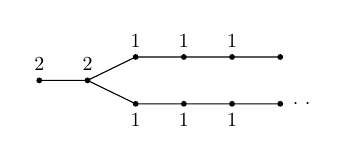
\begin{tikzpicture}[baseline=-.5ex,x=.68cm,y=.62cm]
  \fill (0,0) circle (1.05pt);
  \fill (.9,0) circle (1.05pt);
  \node[above=1pt,scale=.72] at (0,0) {$2$};
  \node[above=1pt,scale=.72] at (.9,0) {$2$};
  \foreach \x/\lab in {1.8/1,2.7/1,3.6/1,4.5/0}{
    \fill (\x,.48) circle (1.05pt);
    \fill (\x,-.48) circle (1.05pt);
    \ifnum\lab=1
      \node[above=1pt,scale=.72] at (\x,.48) {$1$};
      \node[below=1pt,scale=.72] at (\x,-.48) {$1$};
    \fi
  }
  \draw (0,0)--(.9,0)--(1.8,.48)--(4.5,.48);
  \draw (.9,0)--(1.8,-.48)--(4.5,-.48);
  \node[right=2pt,scale=.72] at (4.5,-.48) {$\cdot\ \cdot$};
\end{tikzpicture}
\\

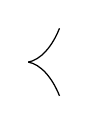
\begin{tikzpicture}[baseline=-.5ex,x=.55cm,y=.55cm]
  \draw[line width=.45pt]
    (0,0) .. controls (.28,.05) and (.55,.35) .. (.72,.78);
  \draw[line width=.45pt]
    (0,0) .. controls (.28,-.05) and (.55,-.35) .. (.72,-.78);
\end{tikzpicture}
& $y^2=x^3$ & $1$ &
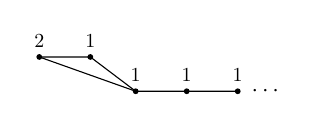
\begin{tikzpicture}[baseline=-.5ex,x=.72cm,y=.65cm]
  \coordinate (A) at (0,.42);
  \coordinate (B) at (.9,.42);
  \coordinate (C) at (1.7,-.25);
  \coordinate (D) at (2.6,-.25);
  \coordinate (E) at (3.5,-.25);
  \foreach \p in {A,B,C,D,E}{\fill (\p) circle (1.05pt);}
  \node[above=1pt,scale=.72] at (A) {$2$};
  \foreach \p in {B,C,D,E}{\node[above=1pt,scale=.72] at (\p) {$1$};}
  \draw (A)--(B)--(C)--(D)--(E);
  \draw (A)--(C);
  \node[right=2pt,scale=.85] at (E) {$\cdots$};
\end{tikzpicture}
\end{tabular}
\end{center}

若 $n>2$，则此图不再确定不变量 $\delta$。例如，三条共点且共面的直线（分别地，不共面的直线）的并，其不变量为 $\delta=3$（分别为 $\delta=2$），而 Enriques 图相同。我不知道这种现象是否也会出现在单支曲线中。

下面给出 $n=3$ 时的两个图的例子，它们不可能由平面曲线产生（参见 2.5）。依次给出曲线的方程、爆破原点后的严格变换的方程、曲线的参数方程、不变量 $\delta$ 和 Enriques 图。

%%%%%%%%%% source scan idx 38 | folio 31 %%%%%%%%%%

\begin{equation}\tag{2.25.1}
\left\{
\begin{gathered}
  \left\{\begin{aligned}y^2&=xz^4,\\ z^3&=x^2,
  \end{aligned}\right.\qquad
  \left\{\begin{aligned}(y/z)^2&=(x/z)^3,\\ z&=(x/z)^2,
  \end{aligned}\right.\\[3pt]
  \left\{\begin{aligned}x&=u^6,\\y&=u^7,\\z&=u^4,
  \end{aligned}\right.\qquad \delta=5
\end{gathered}
\right.
\end{equation}

\begin{center}
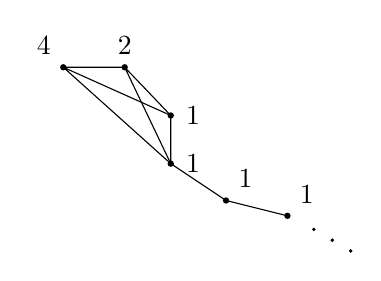
\begin{tikzpicture}[x=.78cm,y=.72cm]
  \coordinate (v1) at (0,0);
  \coordinate (v2) at (1,0);
  \coordinate (v3) at (1.75,-.85);
  \coordinate (v4) at (1.75,-1.70);
  \coordinate (v5) at (2.65,-2.35);
  \coordinate (v6) at (3.65,-2.62);
  \foreach \p in {v1,v2,v3,v4,v5,v6}{\fill (\p) circle (1.15pt);}
  \node[above left=1pt] at (v1) {$4$};
  \node[above=1pt] at (v2) {$2$};
  \node[right=2pt] at (v3) {$1$};
  \node[right=2pt] at (v4) {$1$};
  \node[above right=1pt] at (v5) {$1$};
  \node[above right=1pt] at (v6) {$1$};
  \draw (v1)--(v2) (v1)--(v3) (v1)--(v4);
  \draw (v2)--(v3) (v2)--(v4) (v3)--(v4);
  \draw (v4)--(v5)--(v6);
  \fill (4.08,-2.86) circle (.7pt);
  \fill (4.38,-3.05) circle (.7pt);
  \fill (4.68,-3.24) circle (.7pt);
\end{tikzpicture}
\end{center}

\begin{equation}\tag{2.25.2}
\left\{
\begin{gathered}
  \left\{\begin{aligned}y^2z&=x^3,\\ z^3&=y^2,
  \end{aligned}\right.\qquad
  \left\{\begin{aligned}(y/z)^2&=(x/z)^3,\\ z&=(y/z)^2,
  \end{aligned}\right.\\[3pt]
  \left\{\begin{aligned}x&=u^8,\\y&=u^9,\\z&=u^6,
  \end{aligned}\right.\qquad \delta=10
\end{gathered}
\right.
\end{equation}

\begin{center}
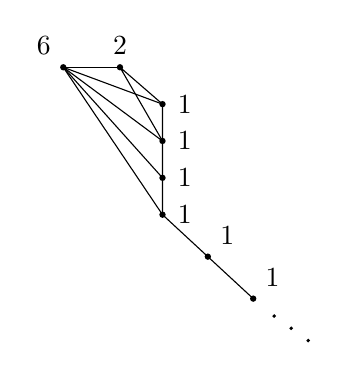
\begin{tikzpicture}[x=.72cm,y=.65cm]
  \coordinate (w1) at (0,0);
  \coordinate (w2) at (1,0);
  \coordinate (w3) at (1.75,-.72);
  \coordinate (w4) at (1.75,-1.44);
  \coordinate (w5) at (1.75,-2.16);
  \coordinate (w6) at (1.75,-2.88);
  \coordinate (w7) at (2.55,-3.70);
  \coordinate (w8) at (3.35,-4.52);
  \foreach \p in {w1,w2,w3,w4,w5,w6,w7,w8}{\fill (\p) circle (1.15pt);}
  \node[above left=1pt] at (w1) {$6$};
  \node[above=1pt] at (w2) {$2$};
  \foreach \p in {w3,w4,w5,w6}{\node[right=2pt] at (\p) {$1$};}
  \node[above right=1pt] at (w7) {$1$};
  \node[above right=1pt] at (w8) {$1$};
  \draw (w1)--(w2);
  \foreach \p in {w3,w4,w5,w6}{\draw (w1)--(\p);}
  \draw (w2)--(w3) (w2)--(w4);
  \draw (w3)--(w4)--(w5)--(w6)--(w7)--(w8);
  \fill (3.72,-4.86) circle (.7pt);
  \fill (4.02,-5.10) circle (.7pt);
  \fill (4.32,-5.34) circle (.7pt);
\end{tikzpicture}
\end{center}
